\chapter{Abschätzung systematischer Unsicherheiten} \label{kap:systematik}
Der Fitter liefert zwar eine statistische Unsicherheit auf $\SJPsi$, allerdings ist eine Betrachtung der Systematik unerlässlich. Im Folgenden wird daher der Einfluss einiger Effekte auf das Fitergebnis untersucht und anschließend der systematische Fehler abgeschätzt.

\section{Fitmethode} \label{kap:fit_bias}
Es ist allgemein bekannt, dass die Parameterabschätzung der Maximum-Likelihood-Methode für eine große Zahl an Messwerten gegen den \glqq wahren Wert\grqq\ konvergiert, für wenig Statistik verfälscht sie jedoch das Ergebnis - sie produziert ein sogenanntes Bias. Um abzuschätzen, ob und in welchem Maße es zu einem Bias kommt, wird eine Toy Monte Carlo - Studie (kurz: Toy MC) durchgeführt. Dabei werden Daten zufällig der Massen- und Eigenzeit-WDF aus Gleichung (\ref{eq:pdf_masse}) bzw. (\ref{eq:fit_pdf}) folgend mit den gewünschten Parametern generiert und im Anschluss gefittet. Zur Generation der Massen- und Eigenzeitverteilung werden die aus den Fits erhaltenen Parameter verwendet (siehe Tabellen \ref{tab:fit_masse} und \ref{tab:fit_results}). Die einzige Ausnahme bildet $\SJPsi$, da diese zum Zeitpunkt dieser Studie noch verdeckt war. Hier wurde mit $\SJPsi = 0,72$, der Resultat der Analyse aus 2011 (\cite{lhcb-paper}), generiert. Entsprechend der Statistik im verwendeten Datensatz werden hier jeweils 20000 Ereignisse generiert. Durch mehrmaliges Wiederholen von Generation und Fit sollten die gefitteten Parameter am Ende mit der Größe des statistischen Fehlers gaußverteilt um die in der Generation verwendeten Parameter sein. Kommt es zu Abweichungen davon, so ist dies auf die Fitmethode oder eine fehlerhafte Implementation des Experimentators zurückzuführen. Um statistisch zuverlässige Aussagen treffen zu können, wurden in dieser Toy MC - Studie insgesamt 20000 Wiederholungen durchgeführt.

\begin{figure}[hptb]
\centering
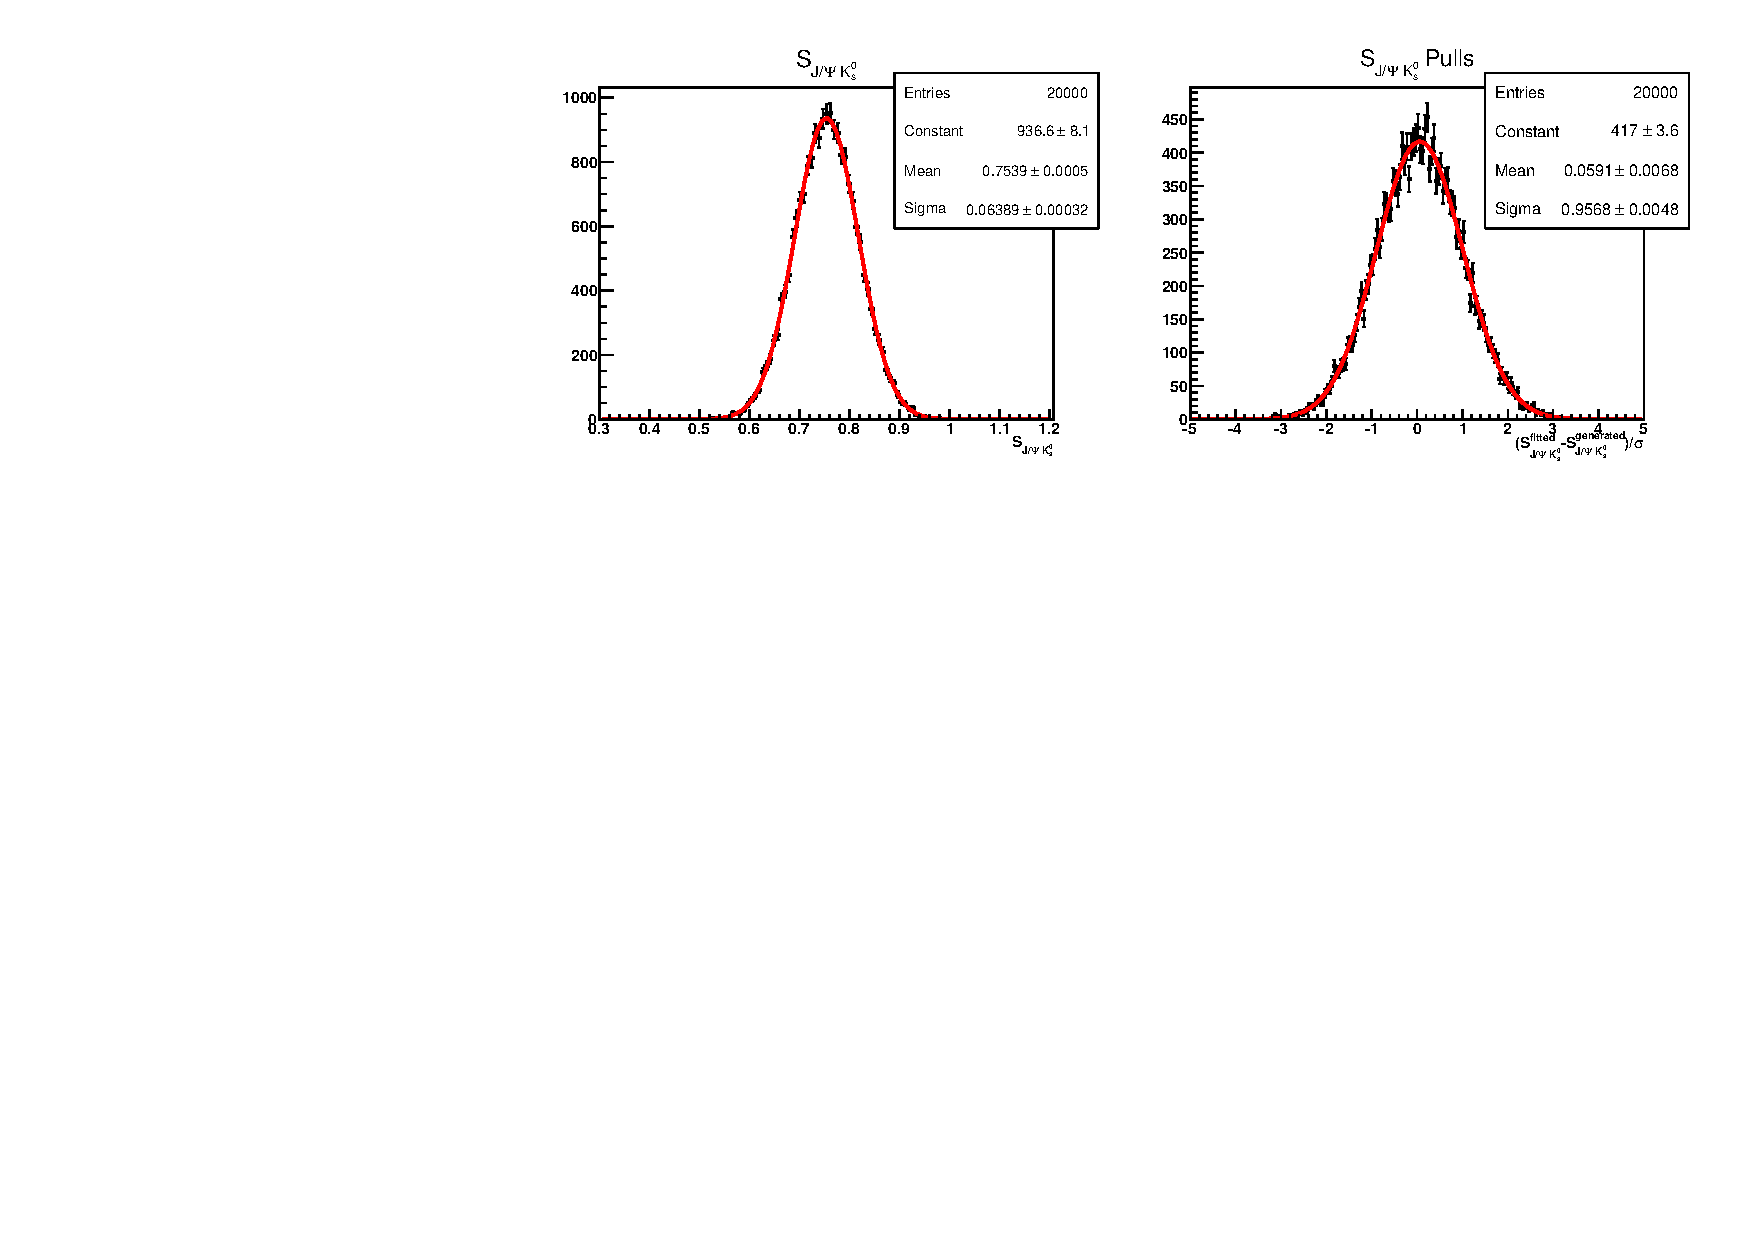
\includegraphics[width = \textwidth]{fit_bias}
\caption{Verteilung der aus der Toy MC Studie erhaltenen Amplituden $\SJPsi$ (links) sowie die dazugehörigen Pulls (rechts)}
\label{fig:fit_bias}
\end{figure}

Abbildung \ref{fig:fit_bias} zeigt sowohl die Verteilung der gefitteten Amplitude $\SJPsi$ als auch die Pulls, die sich mittels $(\SJPsi^{\text{gefittet}} - \SJPsi^{\text{generiert}})/\sigma^{\text{gefittet}}$ berechnen lassen. Der Mittelwert der Amplitudenverteilung (links) $\SJPsi^{\text{ToyMC}} = 0,7234 \pm 0,0004$ weicht signifikant vom generierten Wert $\SJPsi = 0,7200$ ab, es gibt also ein Bias. An der Pull-Verteilung lassen sich prinzipiell zwei Dinge beobachten:
\begin{enumerate}
    \item An der Verschiebung des Pull-Mittelwertes $\mu = 0,0522 \pm 0,0067$ von der Null sieht man deutlich, dass es - wie bereits erwähnt - einen kleinen, aber signifikanten Bias gibt. Indem dieser Bias mit der statistischen Unsicherheit aus dem Fitergebnis (siehe Gl. \ref{eq:fit_result}) multipliziert wird, erhält man eine Abschätzung der aus der Fitmethode resultierenden Unsicherheit:
        \begin{align}
        \delta\SJPsi^{Fit} = 0,0522 \cdot 0,0626 = 0,0033
        \end{align}

    \item Mit einem $\sigma = 0,941 \pm 0,005$ ist die Pull-Verteilung signifikant zu schmal. Bei einer zufälligen Streuung der Werte wird $\sigma=1$ erwartet. Dies bedeutet, dass der Fit den statistischen Fehler um $5,6\%$ überschätzt. Dieses Ergebnis kann später als Faktor zur Korrektur des statistischen Fehlers verwendet werden. 
\end{enumerate}

\subsubsection{Ursachen des Bias und der Fehlerüberschätzung}
Es bleibt zu klären, welche Ursachen zu dem Bias und der Fehlerüberschätzung führen. Wie bereits erwähnt, verfälscht die Likelihood-Methode für zu wenige Messwerte / Ereignisse die Parameterabschätzung. Demnach liegt die Vermutung nahe, dass im vorliegenden Datensatz zu wenig Ereignisse (\glqq Statistik\grqq) vorhanden sind. Daher wurden weitere Toy MC Studien mit unterschiedlicher Anzahl an Teilchen pro Toy durchgeführt. Die Ergebnisse sind in Tabelle \ref{tab:fit_bias_events} aufgeführt und in Abbildung \ref{fig:fit_bias_events} nochmals visualisiert. Man sieht, dass das Bias mit erhöhter Statistik deutlich reduziert wird und damit zu wenig Statistik als Hauptursache hierfür angesehen werden kann.

Die Fehlerüberschätzung tritt auf, sobald man in den Toys Untergrund miteinbezieht (ohne Untergrund erhält man ein $\sigma=1,007\pm 0,005$ und ist damit kompatibel zur Eins). Es ist bekannt, dass die verwendete sFit-Methode die Fehlerpropagation (gerade bei Untergrund) nicht korrekt ausführt. Es wurde vom Betreuer eine Fehlerkorrektur implementiert, dabei handelt es sich jedoch um eine Näherung. Für eine tiefergehende Studie müsste die Fehlerkorrektur entsprechend analysiert werden.

\begin{table}[hptb]
\centering
\caption{Toy MC Studien mit unterschiedlicher Anzahl an generierten Ereignissen pro Toy. Genannt wird der Mittelwert $\mu$ der $\SJPsi$-Pull-Verteilung}
\label{tab:fit_bias_events}
\begin{tabular}{cr@{$\pm$}l}
\hline \hline 
Teilchen pro Toy & \multicolumn{2}{c}{$\mu$}  \\ \hline
20000            &  0,0522 & 0,0067 \\
50000            &  0,0358 & 0,0067 \\
100000           &  0,0257 & 0,0068 \\
200000           &  0,0145 & 0,0068 \\ 
\hline \hline
\end{tabular}
\end{table}

\begin{figure}[hptb]
\centering
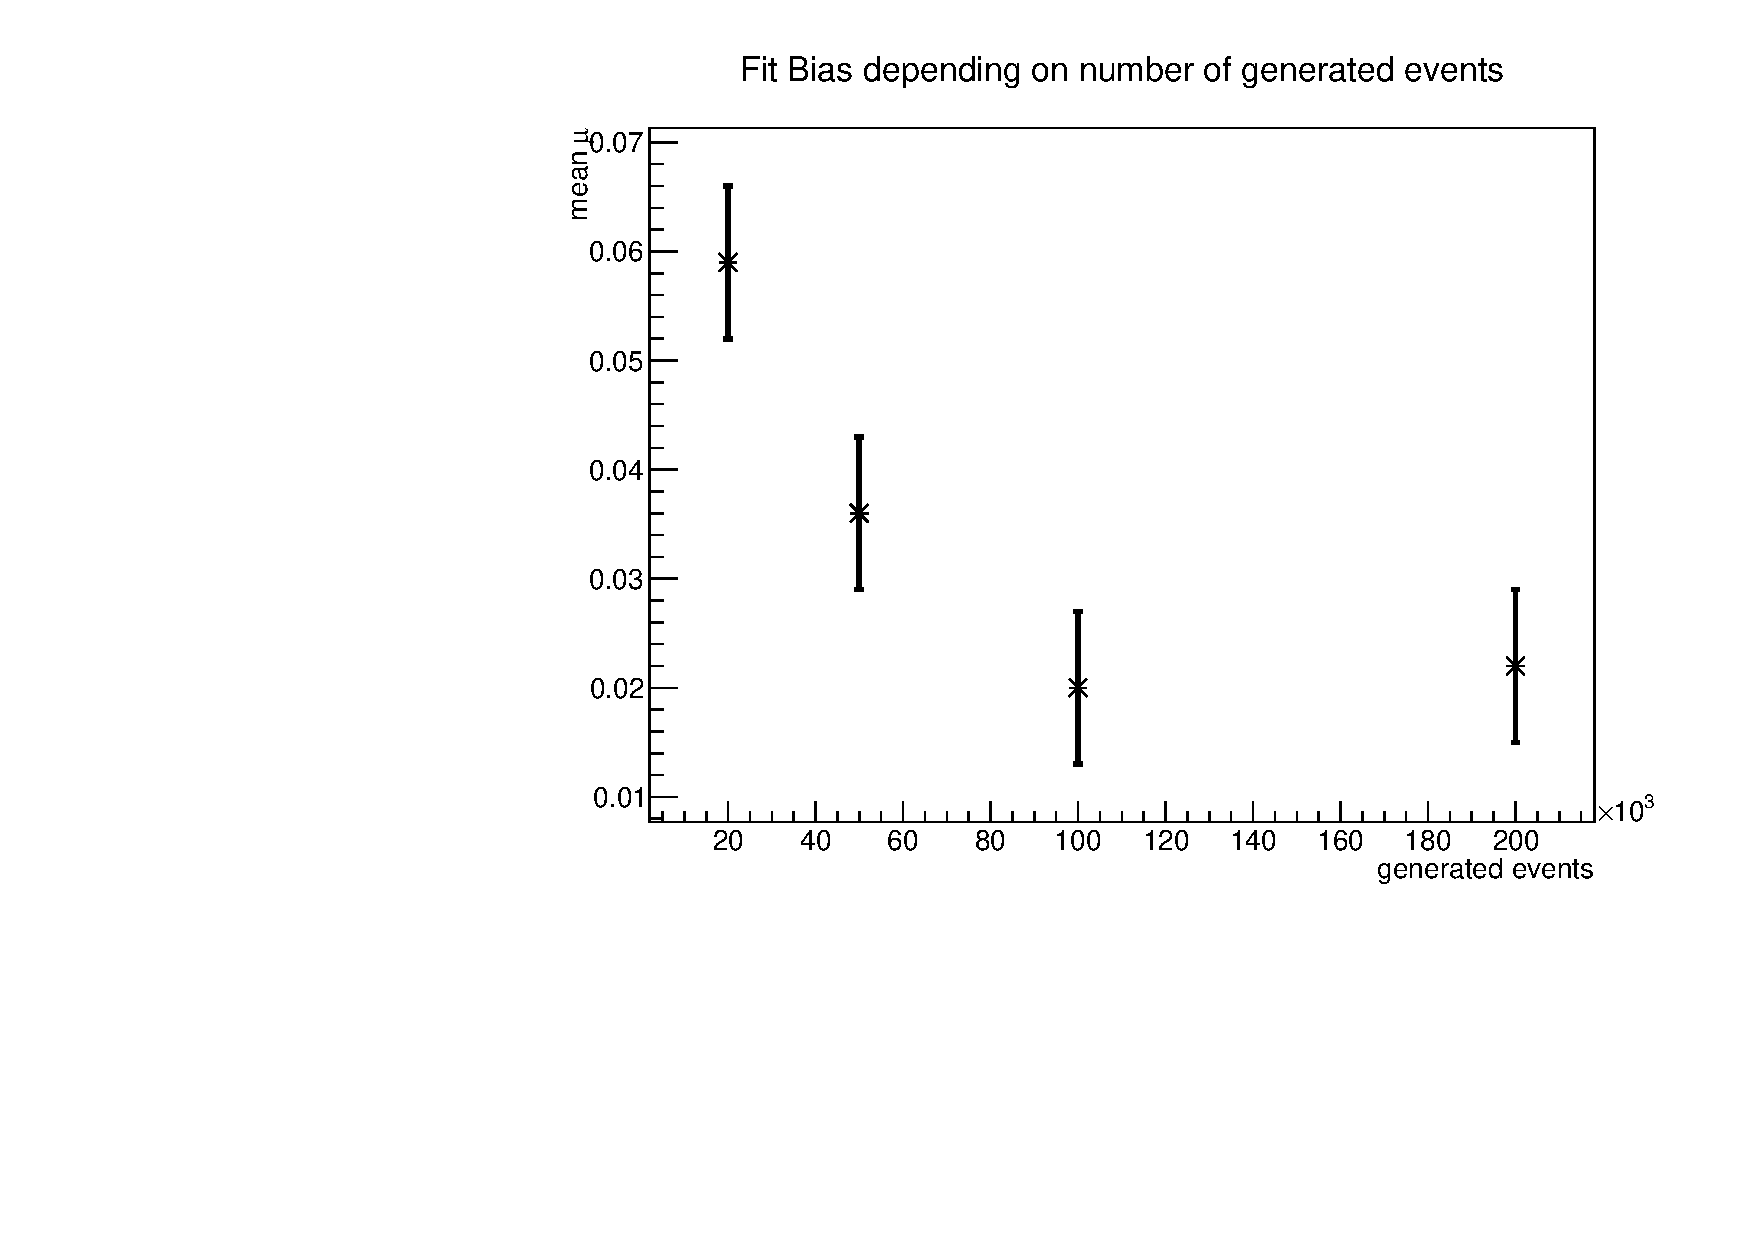
\includegraphics[width=\textwidth]{fit_bias_statistics}
\caption{Toy MC Studien mit unterschiedlicher Anzahl an generierten Ereignissen pro Toy. Als Maß für das Fit Bias dient der Mittelwert $\mu$ der $\SJPsi$-Pull-Verteilung}. Der erste Eintrag entspricht der in Daten vorliegenden Statistik.
\label{fig:fit_bias_events}
\end{figure}

\section{Kalibration der Flavour-Tagging-Algorithmen}
Im Fit wird bei den Parametern der Tagging Kalibration durch \glqq gaußische\grqq\ Einschränkung der Parameter deren statistische Fehler berücksichtigt. Bislang unbeachtet blieben die systematischen Fehler von $p_0$ und $p_1$, deren Einfluss im Folgenden untersucht wird. Leider sind die externen Studien zur Systematik des in dieser Analyse verwendeten Flavour-Taggings noch nicht abgeschlossen, sodass die systematischen Fehler $\delta p_0^{\text{stat.}}$ sowie $\delta p_1^{\text{stat.}}$ noch nicht vorliegen. Um dennoch ein Gefühl für den Einfluss des Flavour-Taggings zu bekommen, werden die systematischen Fehler der 2011-Analyse (\cite{lhcb-paper}) herangezogen. Die Annahme und Erwartung ist, dass sich die Systematiken zwischen 2011 und 2012 kaum unterscheiden. Für eine endgültige Analyse, muss dieser Schritt jedoch wiederholt werden, sobald die Analyse des Flavour-Taggings aus 2012 abgeschlossen ist. In dieser Arbeit werden nun folgende Werte und Fehler der Kalibrationsparameter $p_0$ und $p_1$ verwendet:
\begin{align}
p_0 &= 0,382 \pm 0,003\ \text{(stat.)} \pm 0,008\ \text{(syst.)}, \\
p_1 &= 0,981 \pm 0,024\ \text{(stat.)} \pm 0,012\ \text{(syst.)}.
\end{align}

\subsubsection{Variation der Parameter in den Daten}
Einen ersten Überblick über die Systematik erhält man, indem man
im regulären Eigenzeitfit die Startwerte der Parameter $p_0$ und $p_1$ um ihre systematischen Fehler variiert. In allen vier möglichen Kombinationen wird der systematische Fehler auf $p_0$ und $p_1$ addiert bzw. subtrahiert, dann der Fit durchgeführt und schließlich die Abweichung vom regulären Fitergebnis für $\SJPsi$ berechnet. Der verdeckte Referenzwert aus dem Fit beträgt
\begin{align}
\SJPsi = 0,5347 \pm 0,0626 
\end{align}

\begin{table}[hptb]
\centering
\caption{Variation des Fitergebnisses für $\SJPsi$ bei Veränderung der Startwerte für $p_0$ und $p_1$ $\pm$ ihrer systematischen Unsicherheiten}
\label{tab:syst_fit_calib_data}
\begin{tabular}{cc|r@{$\pm$}l|r}
\hline\hline
$p_0$  &  $p_1$  &  \multicolumn{2}{c|}{$\SJPsi$}  & $\Delta\SJPsi$   \\ \hline
0,382 - 0,008  &  0,981 - 0,024  &  0,5109 & 0,0604  &  -0,0238 \\
0,382 - 0,008  &  0,981 + 0,024  &  0,5103 & 0,0604  &  -0,0244 \\
0,382 + 0,008  &  0,981 - 0,024  &  0,5599 & 0,0649  &   0,0252 \\
0,382 + 0,008  &  0,981 + 0,024  &  0,5591 & 0,0648  &   0,0244 \\
\hline\hline
\end{tabular}
\end{table}

Die Ergebnisse sind Tabelle \ref{tab:syst_fit_calib_data} zu entnehmen. Die größte Abweichung beträgt hier $\Delta\SJPsi = 0,0252$.

\subsubsection{Variation der Parameter in Toy MC}
Eine weitere Möglichkeit der Abschätzung besteht darin, sich entsprechende Toys mit verfälschten $p_0$ und $p_1$ zu generieren und diese dann normal zu fitten. Im Folgenden werden bei der Generation der Toys die Parameter $p_0$ und $p_1$ um ihre systematischen Unsicherheiten variiert, der Fit dann allerdings mit den ursprünglichen Parameterwerten durchgeführt. Als Referenzwert dient die Toy MC Studie aus Kapitel \ref{kap:fit_bias}, da dort mit den regulären Parametern $p_0$ und $p_1$ generiert und gefittet wurde. Jene Amplitude betrug
\begin{align}
\SJPsi = 0,7234 \pm 0,0004.
\end{align}

\begin{table}[hptb]
\centering
\caption{Variation des Fitergebnisses für $\SJPsi$ bei Veränderung der Parameterwerte $p_0$ und $p_1$ $\pm$ ihrer systematischen Unsicherheiten bei der Generation von Toys}
\label{tab:syst_fit_calib_toys}
$\begin{array}{cc|r@{\pm}l|r}
\hline\hline
p_0  &  p_1  &  \multicolumn{2}{c|}{\SJPsi}  & \Delta\SJPsi   \\ \hline
0,382 - 0,008  &  0,981 - 0,024  &  0,7515 & 0,0004  &   0,0281 \\
0,382 - 0,008  &  0,981 + 0,024  &  0,7565 & 0,0004  &   0,0331 \\
0,382 + 0,008  &  0,981 - 0,024  &  0,6909 & 0,0004  &  -0,0325 \\
0,382 + 0,008  &  0,981 + 0,024  &  0,6966 & 0,0004  &  -0,0244 \\
\hline\hline
\end{array}$
\end{table}

Die Ergebnisse sind Tabelle \ref{tab:syst_fit_calib_toys} zu entnehmen, die dazugehörigen Plots werden in Abbildung \ref{fig:toys_tag_calib} gezeigt. Die größte Abweichung beträgt hier $\Delta\SJPsi = 0,0331$ und ist auch größer als bei Variation der Parameter in den Daten. Dementsprechend wird der systematische Fehler durch die Tagging Kalibrierung mit ebendiesem Wert konservativ abgeschätzt:

\begin{align}
\delta\SJPsi^{\text{FTK}} = 0,0331\ .
\end{align}

\begin{figure}[hptb]
\centering
\subfigure[{$p_0 - \Delta p_0$,  $p_1 - \Delta p_1$}]{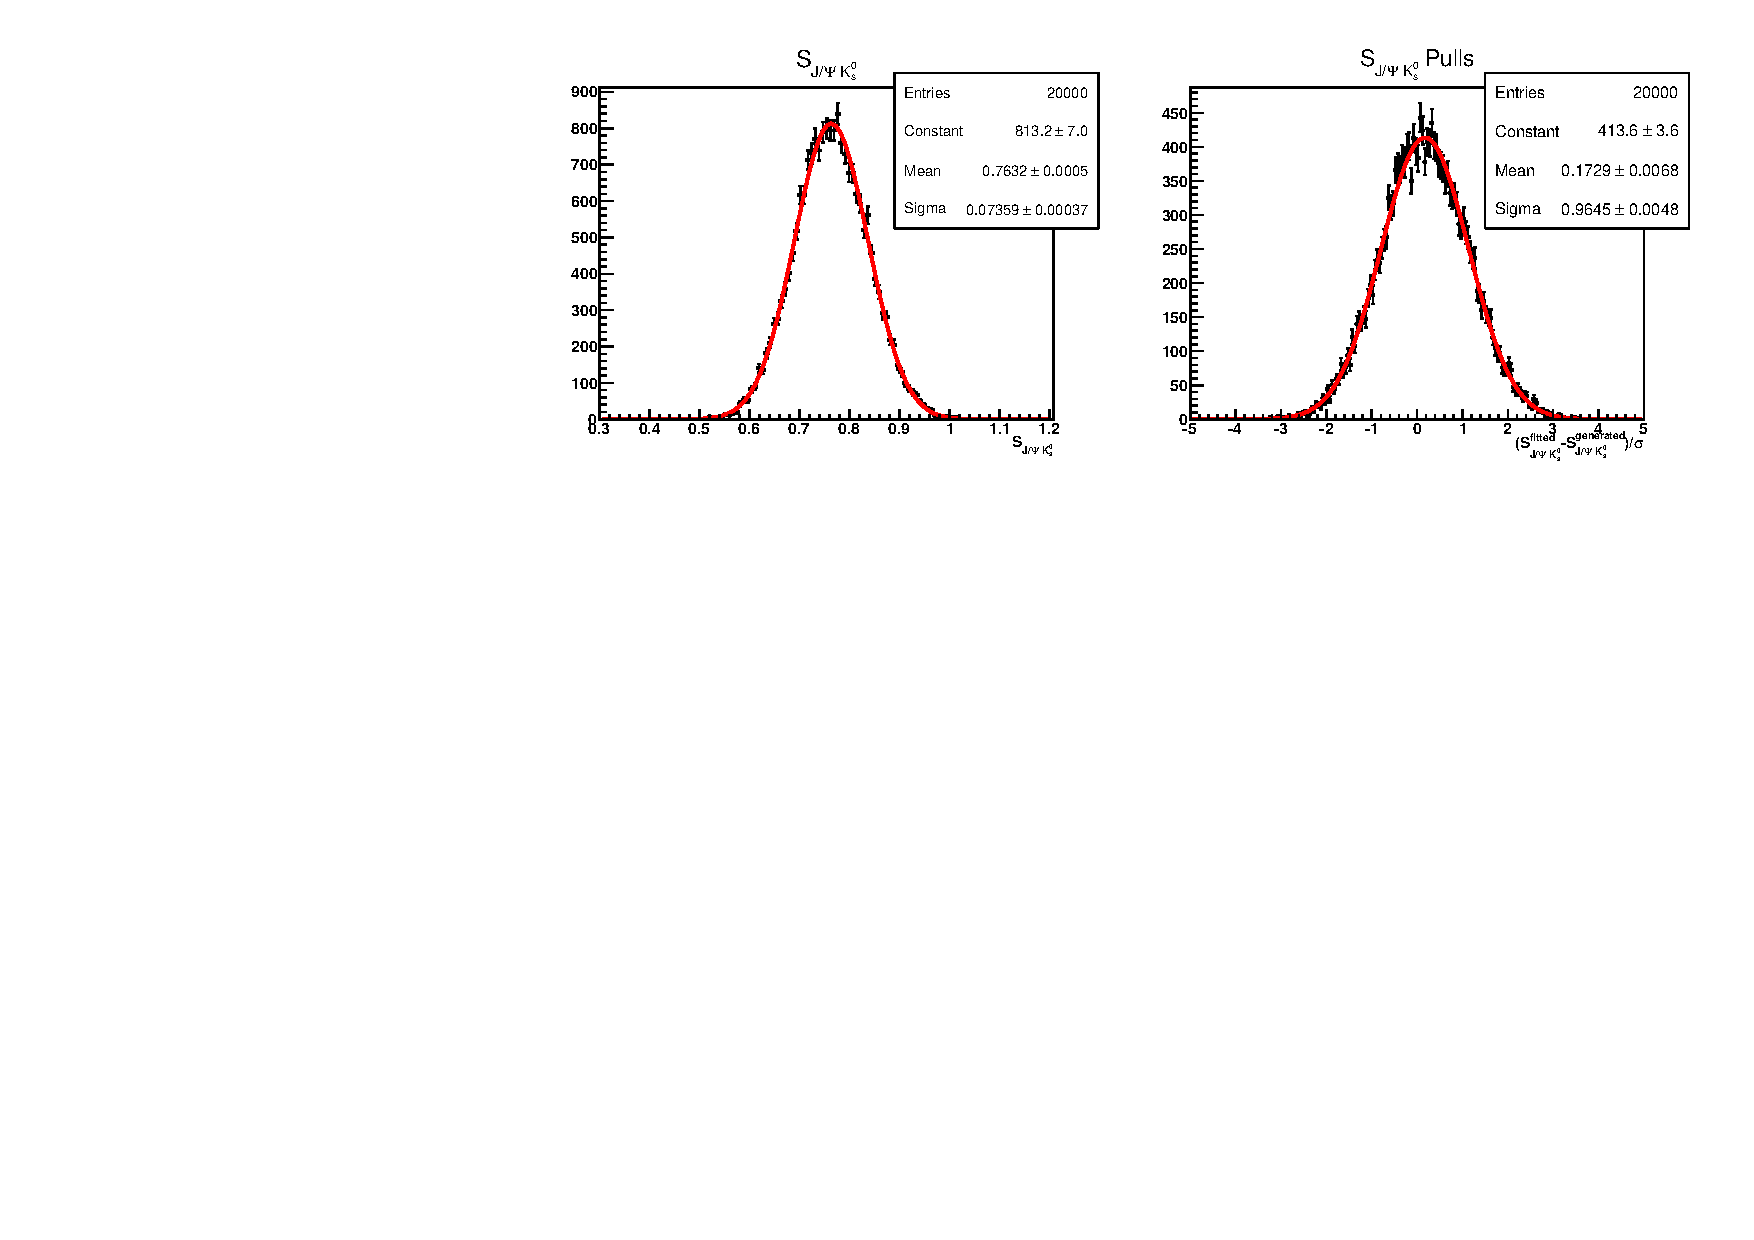
\includegraphics[width=0.7\textwidth]{tagging_calibration--}}
\subfigure[{$p_0 + \Delta p_0$,  $p_1 - \Delta p_1$}]{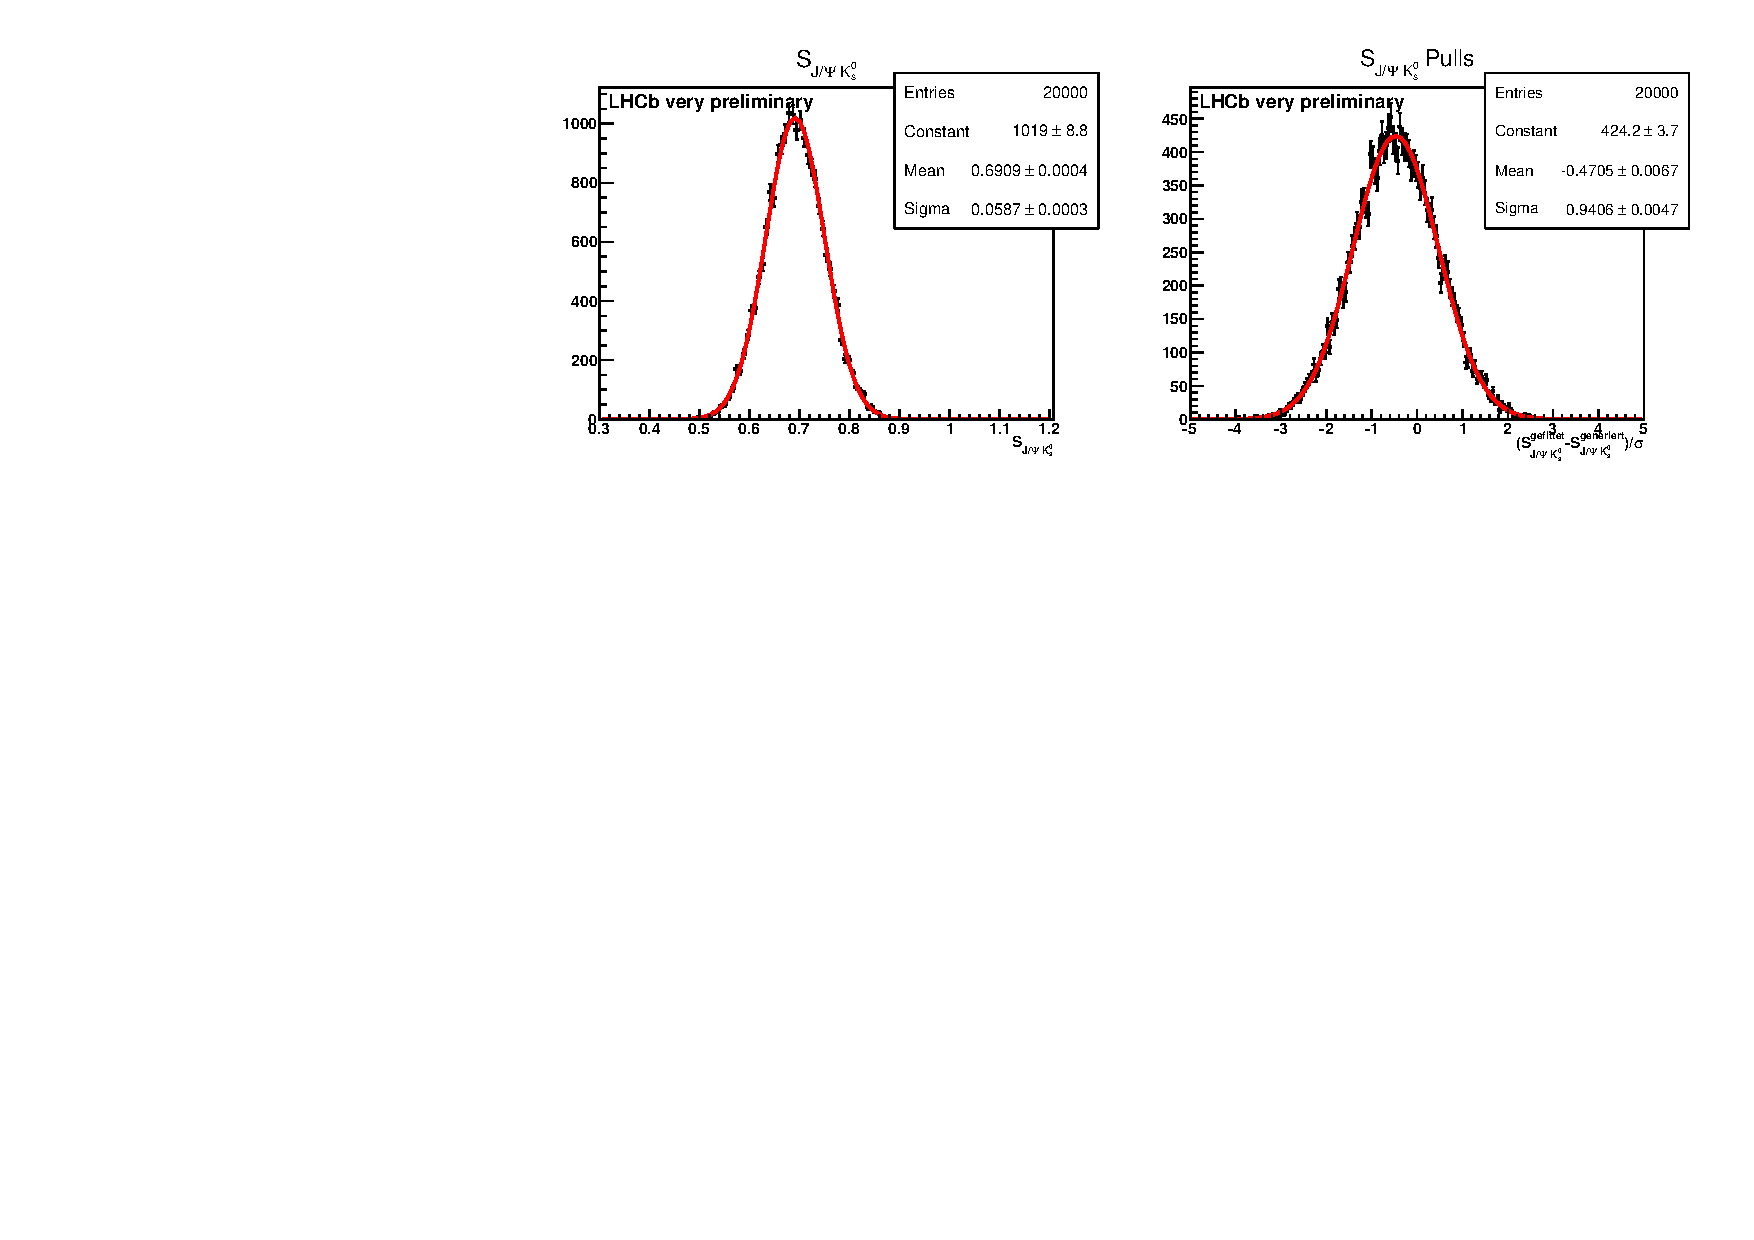
\includegraphics[width=0.7\textwidth]{tagging_calibration+-}}
\subfigure[{$p_0 - \Delta p_0$,  $p_1 + \Delta p_1$}]{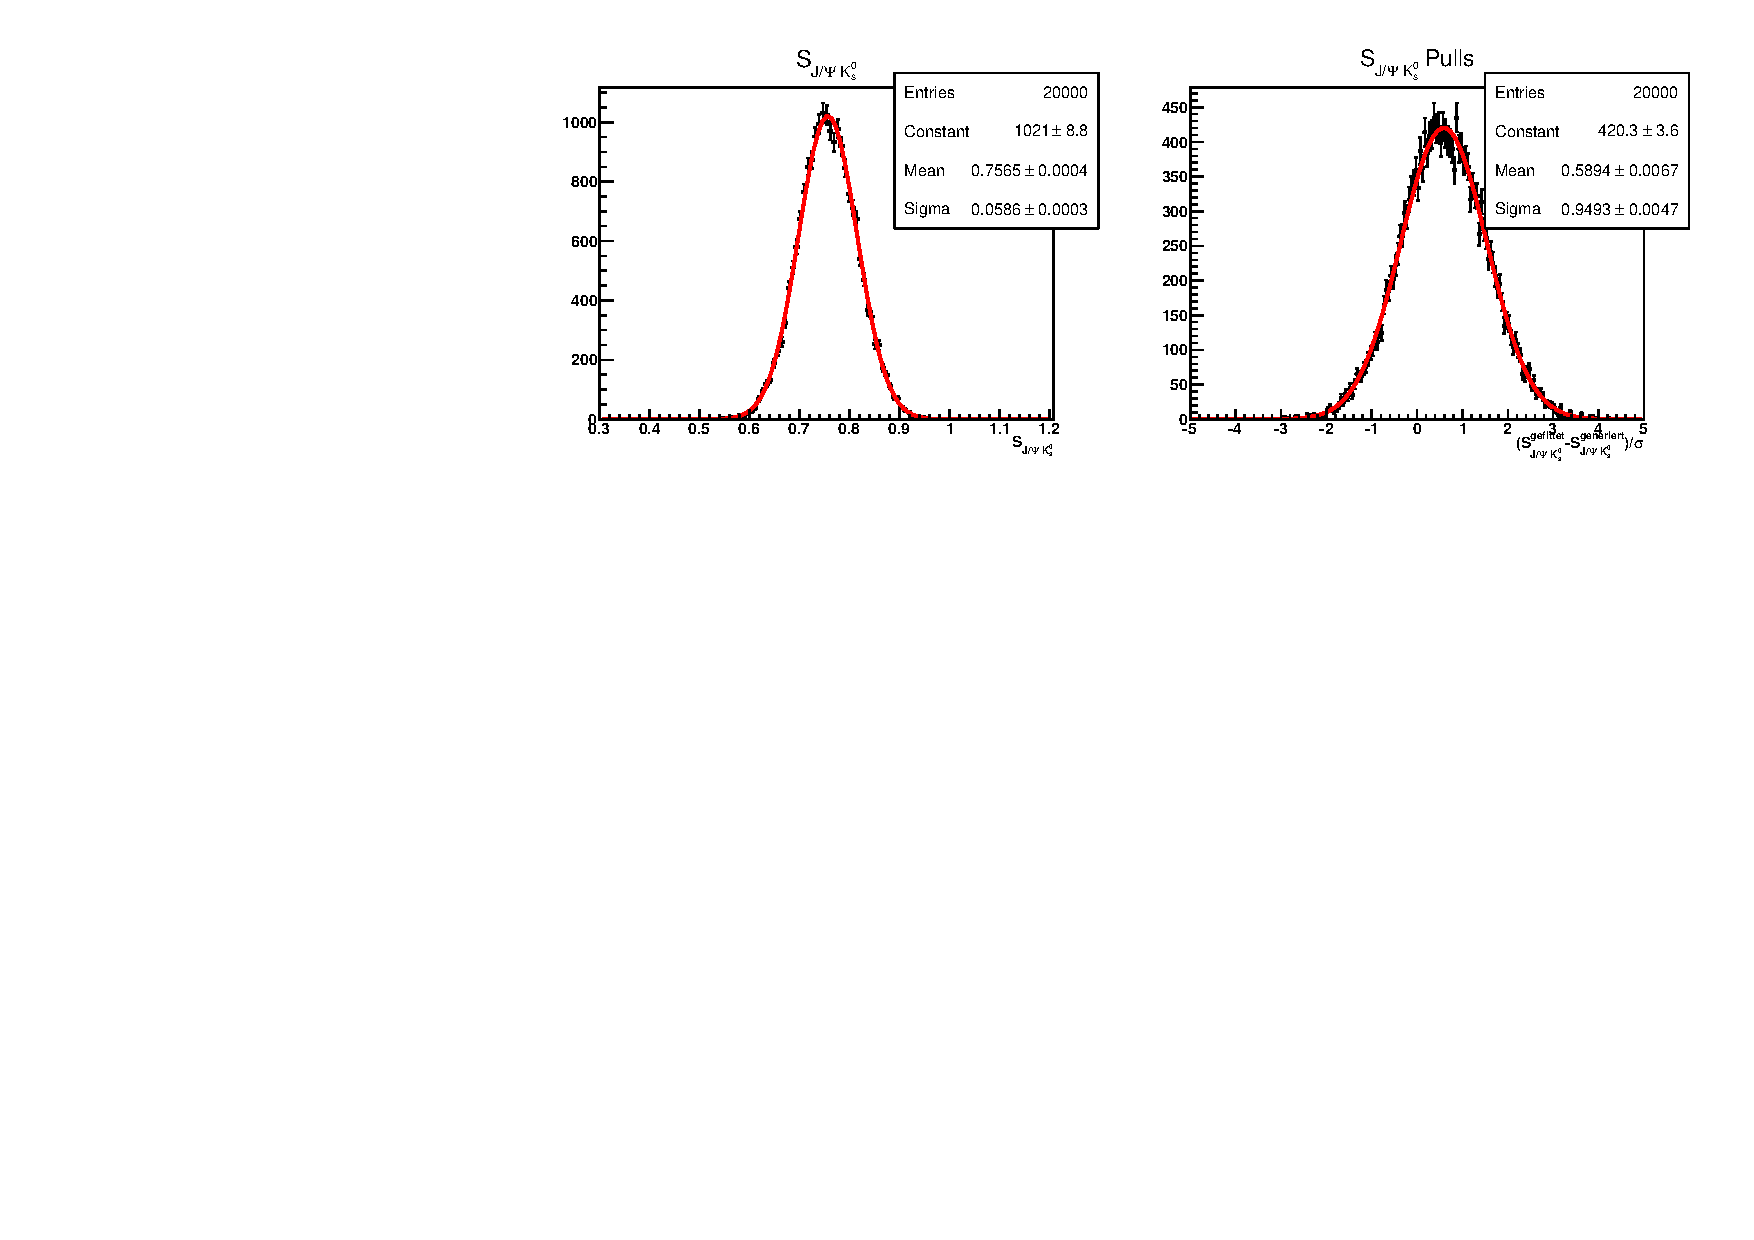
\includegraphics[width=0.7\textwidth]{tagging_calibration-+}}
\subfigure[{$p_0 + \Delta p_0$,  $p_1 + \Delta p_1$}]{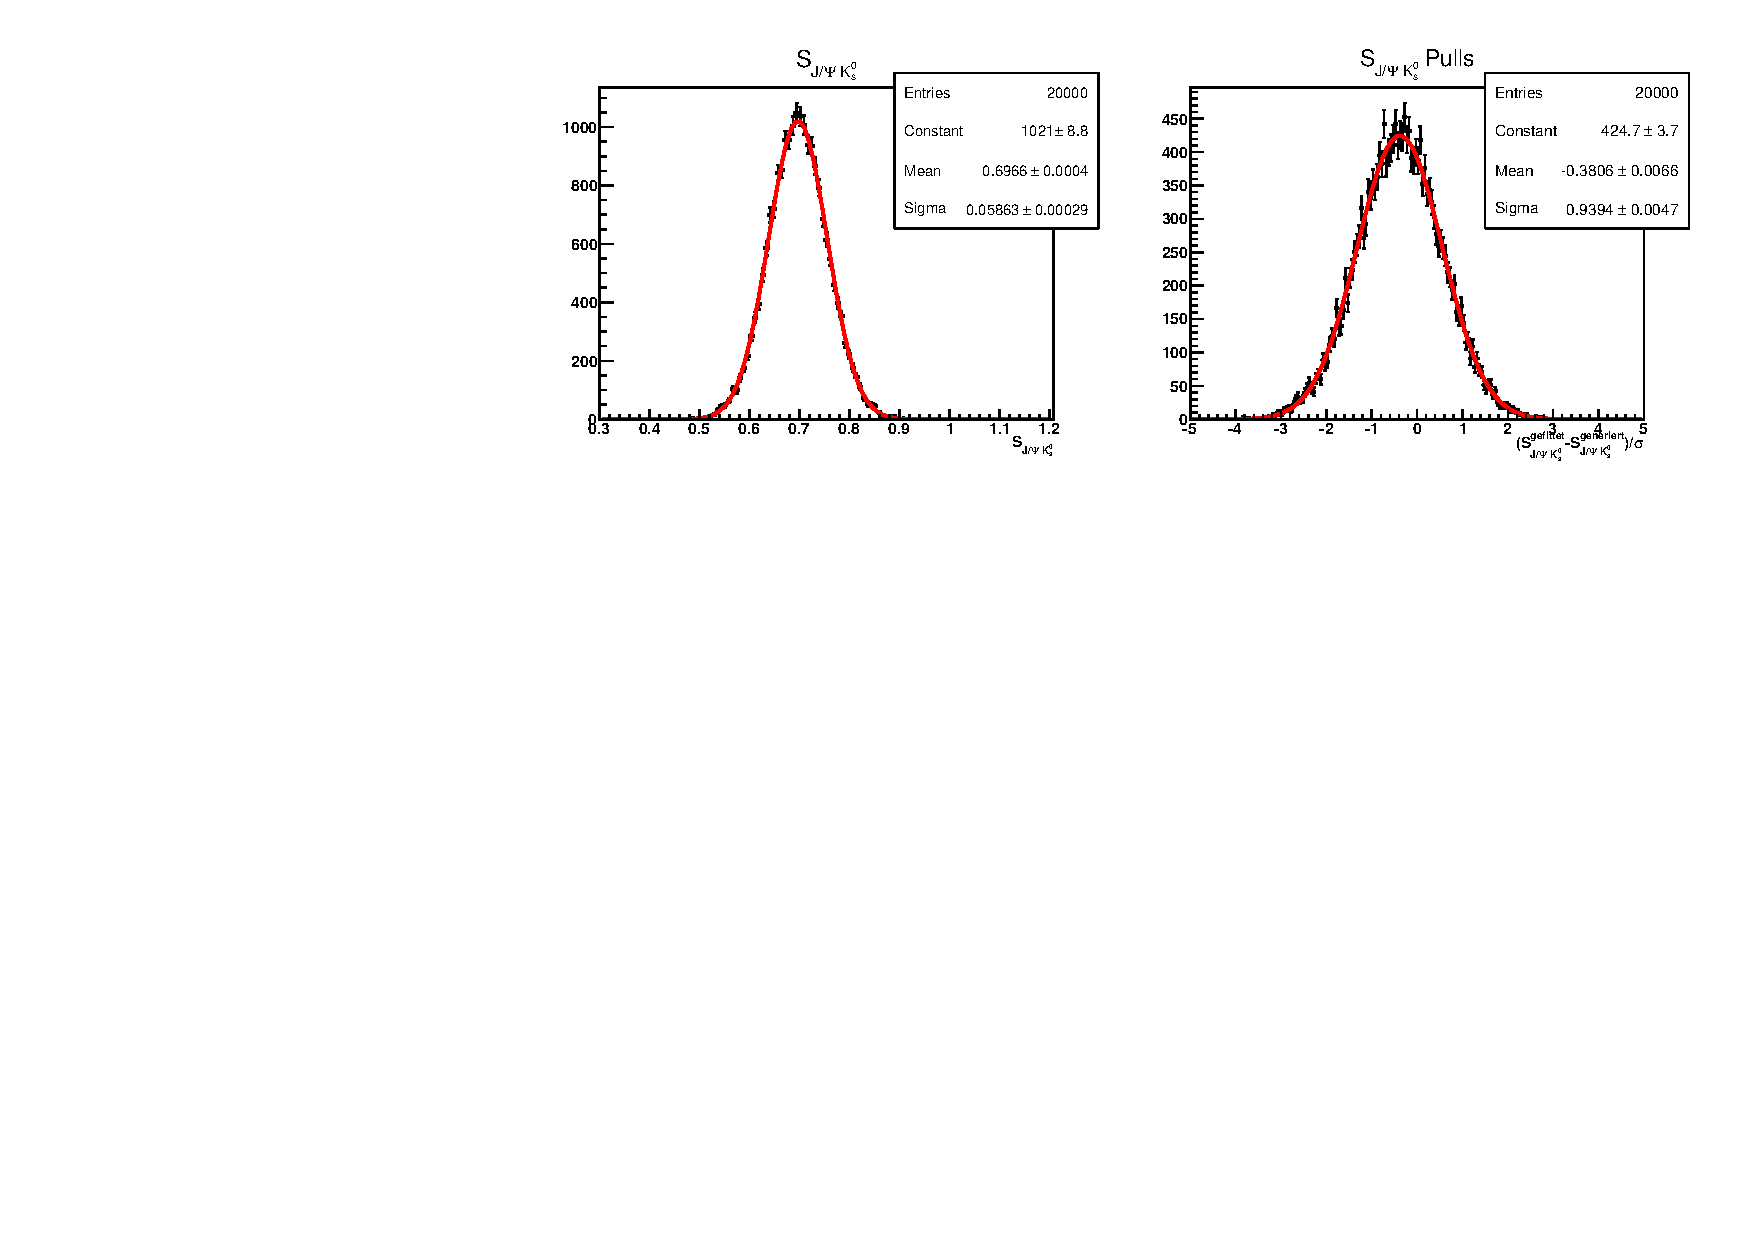
\includegraphics[width=0.7\textwidth]{tagging_calibration++}}
\caption{Toy MC Studie zur Abschätzung der Systematik durch die Tagging Kalibration. Bei der Generation wurden die Taggingparameter $p_0=0,382$ und $p_1=0,981$ um ihre systematischen Unsicherheiten $\Delta p_0 = 0,008$ bzw. $\Delta p_1 = 0,024$ variiert, der Fit wurde dann mit den ursprünglichen Werten $p_0$ und $p_1$ durchgeführt.}
\label{fig:toys_tag_calib}
\end{figure}


\section{Einfluss einer zeitabhängigen Akzeptanz} \label{kap:akzeptanz}
In der Analyse wurde der Einfluss einer zeitabhängigen Detektorakzeptanz vernachlässigt. Nimmt man an, dass sich die Akzeptanz von \Bd- und \Bdbar-Mesonen nicht unterscheiden, so hat die Akzeptanz keinen Einfluss auf die \CP-Asymmetrie nach Gleichung \ref{eq:cp_asymm}, da sie sich hier herauskürzt. Beim Fit der Amplitude nach Gleichung \ref{eq:fit_pdf} ist dies aber nicht zwangsläufig so. Um die Vernachlässigung einer zeitabhängigen Akzeptanz zu rechtfertigen, wird zunächst eine Bestimmung der Akzeptanz durchgeführt und anschließend mit einer Toy MC Studie ihr Einfluss überprüft.

\subsubsection{Bestimmung einer Akzeptanzfunktion} 
\Bd-Mesonen haben eine relativ lange Lebensdauer. Um sie von kurzlebigem Untergrund zu unterscheiden, befinden sich auf den Triggern und dem Stripping entsprechende Selektionen auf die Signifikanz der Zerfallslänge. Dies hat zur Folge, dass für kleine Flugzeiten ($t \lesssim 0,3\pico\second$) kaum \Bd-Mesonen im Detektor registriert werden. Es hat sich herausgestellt \cite{lhcb-paper}, dass dieser Effekt gut durch die Funktion
\begin{align}
\epsilon_1(t) = \frac{2}{\pi}\arctan[t\cdot \exp(at+b)]
\end{align}
parametrisiert werden kann.

Je länger ein \Bd-Meson lebt, desto schwieriger wird es, diese Zerfallsprodukte im Detektor auf Grund seiner Geometrie nachzuweisen. Daher nimmt die Akzeptanz zu großen Zeiten hin wieder ab. Zur Parametrisierung fällt die Wahl auf eine lineare Funktion
\begin{align}
\epsilon_2(t) = 1 + \beta t \qquad (\beta < 0).
\end{align}
Die entsprechende gesamte Akzeptanzfunktion lautet demnach:
\begin{align}
\epsilon(t) = \epsilon_1(t) \cdot \epsilon_2(t) = \frac{2}{\pi}\arctan[t\cdot \exp(at+b)](1 + \beta t)
\end{align}
Zur Bestimmung der Parameter wird die Trennung von \Bd- und \Bdbar-Mesonen aufgehoben, sodass lediglich ein exponentieller Zerfall zu beobachten ist. Des weiteren wird die Selektion der Lebensdauer bei $0,3\pico\second$ nicht angewandt, sodass die Akzeptanz bei kleinen Eigenzeiten sichtbar wird. Die Wahrscheinlichkeitsdichtefunktion für den Fit lautet somit:
\begin{align}
\mathcal{P}_{acc}(t) \propto \epsilon(t)\cdot \e^{-t/\tau} = \e^{-t/\tau}\cdot\frac{2}{\pi}\arctan[t\cdot \exp(at+b)](1 + \beta t)
\end{align}
Die beiden Parameter $\tau$ und $\beta$ sind stark miteinander korreliert. Für eine geeignete Bestimmung der Parameter der Akzeptanz-Funktion wird daher die Lebensdauer auf den PDG-Wert $\tau = 1,519 \pm 0,007 \pico\second$ \cite{pdg-tau} gaußisch eingeschränkt, die anderen Parameter sind frei. Die Ergebnisse sind in Tabelle \ref{tab:fit_akzeptanz} aufgeführt, die entsprechenden Plots in Abbildung \ref{fig:fit_akzeptanz}. 

\begin{table}[hptb]
\centering
\caption{Ergebnis des Fits zur Bestimmung der zeitlichen Akzeptanz. $\tau$ wurde auf den PDG-Wert $\tau = 1,519 \pm 0,007 \pico\second$ \cite{pdg-tau} gaußisch eingeschränkt.}
\label{tab:fit_akzeptanz}
\begin{tabular}{lr@{$\pm$}ll}
\hline \hline 
Parameter & \multicolumn{2}{c}{Ergebnis} & \\ \hline
$\tau$    &  (1,519   & 0,007) & $\ps$ \\
$a $       &  (47,9    & 5,6) & $\ps^{-1}$ \\
$b$       &  -8,4    & 1,1 \\
$\beta$   &  (-0,0090 & 0,0076) & $\ps^{-1}$ \\ 
\hline \hline
\end{tabular}
\end{table}

\begin{figure}[hptb]
\centering
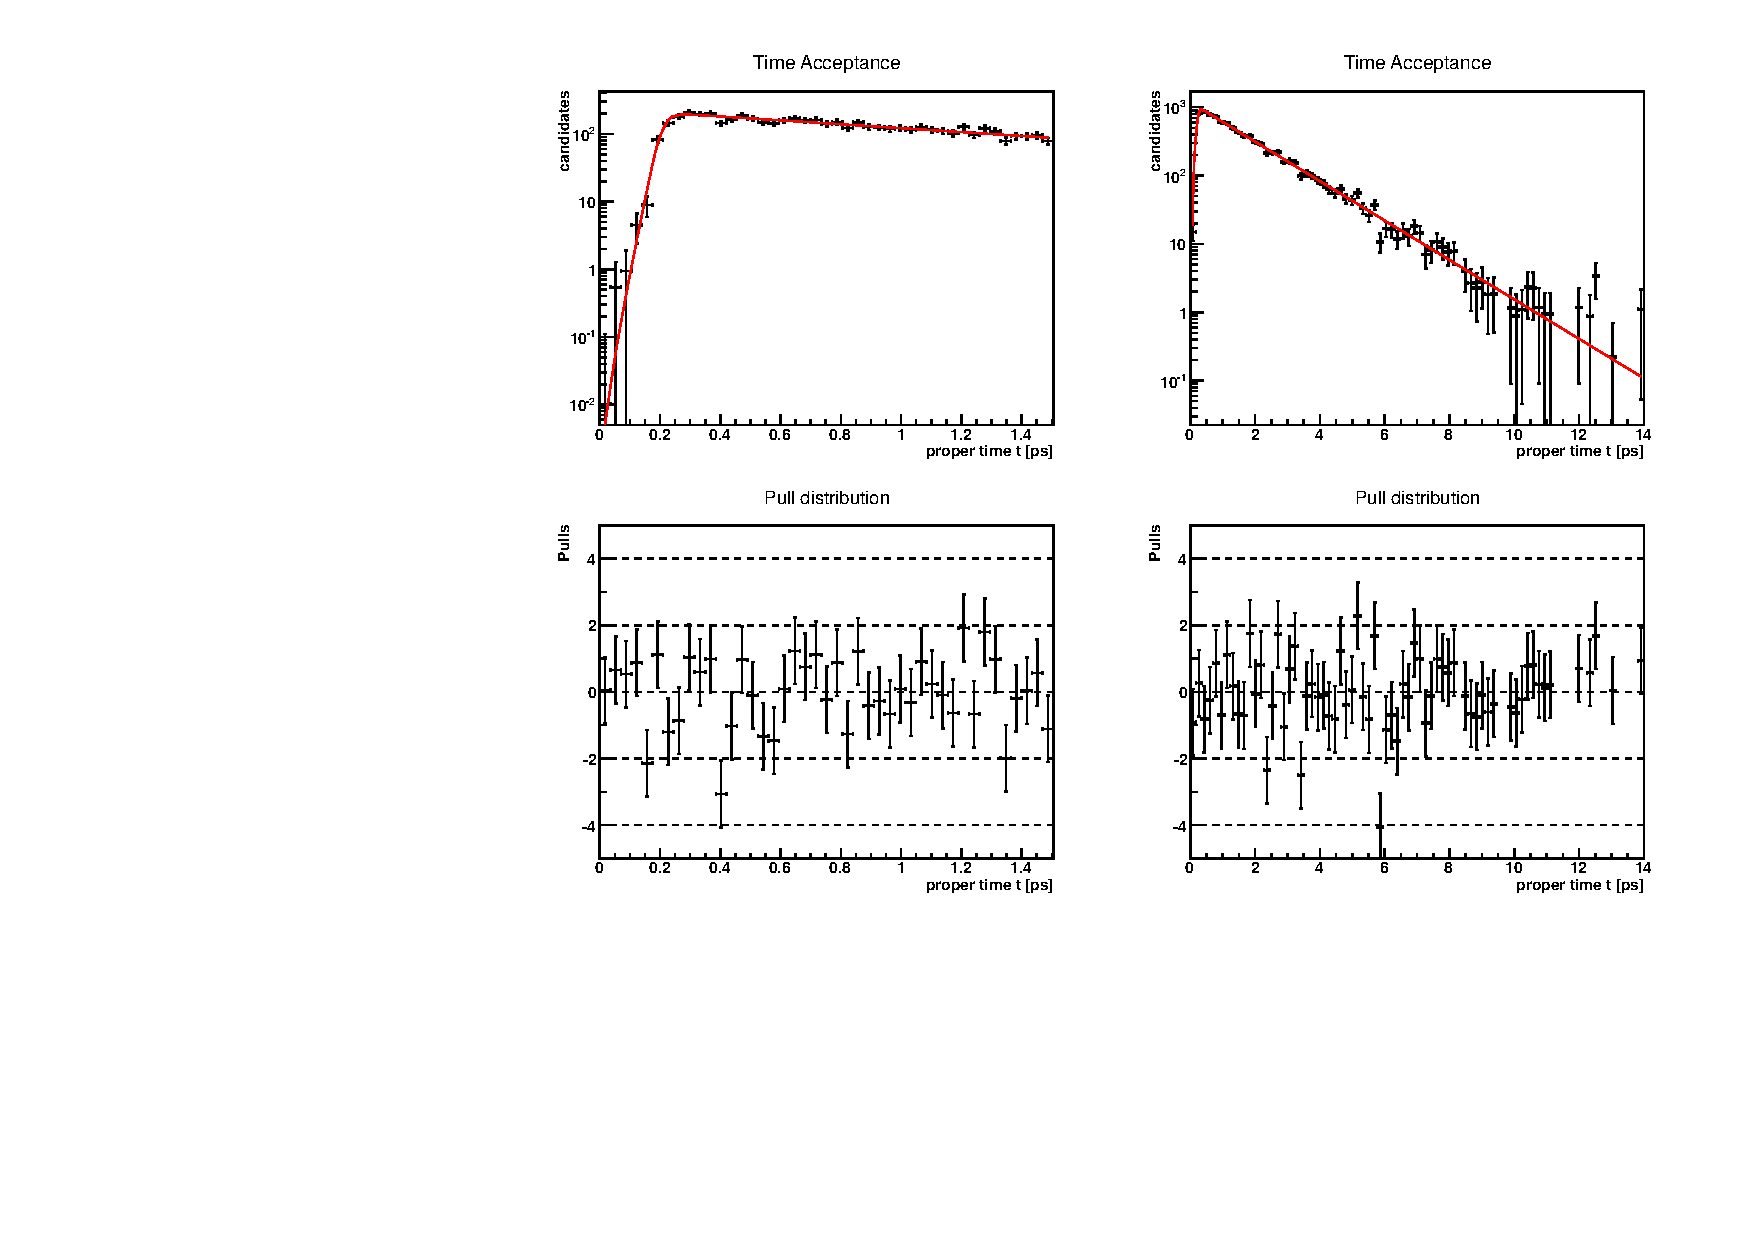
\includegraphics[width=\textwidth]{time_acceptance_fit}
\caption{Fit an die Eigenzeit-Verteilung aller \Bd-Mesonen mit eingeschlossener Akzeptanzfunktion (oben) sowie die entsprechende Pull-Verteilung (unten). Links: kurzlebiger Zeitbereich ($t<1,5\pico\second$), Rechts: gesamtes Eigenzeitspektrum ($0\ps < t < 14\ps$)}
\label{fig:fit_akzeptanz}
\end{figure}

\subsubsection{Bestimmung des Einflusses}
Durch die Selektion der Eigenzeit ab $t = 0,3\ps$ in der Datenselektion spielt die Akzeptanz für kleine Eigenzeiten kaum eine Rolle Dies wird dadurch deutlich, dass die Akzeptanzfunktion $\epsilon(0,3\ps) = 0,992$ und damit fast Eins ist. In der Analyse aus 2011 \cite{lhcb-paper} wurde nur ein geringer Effekt auf das Fitergebnis beobachtet. Dies soll nun verifiziert und das Vorgehen, im Eigenzeitfit die zeitliche Detektorakzeptanz zu vernachlässigen, gerechtfertigt werden. Mit den oben bestimmten Parametern wird die zeitliche Akzeptanz bei der Erzeugung von Daten einer weiteren Toy MC Studie berücksichtigt, der anschließende Fit aber ohne Akzeptanzfunktion durchgeführt. Die zur Erzeugung verwendeten Parameter entsprechen ansonsten denen in Kapitel \ref{kap:fit_bias}.

\begin{figure}[hptb]
\centering
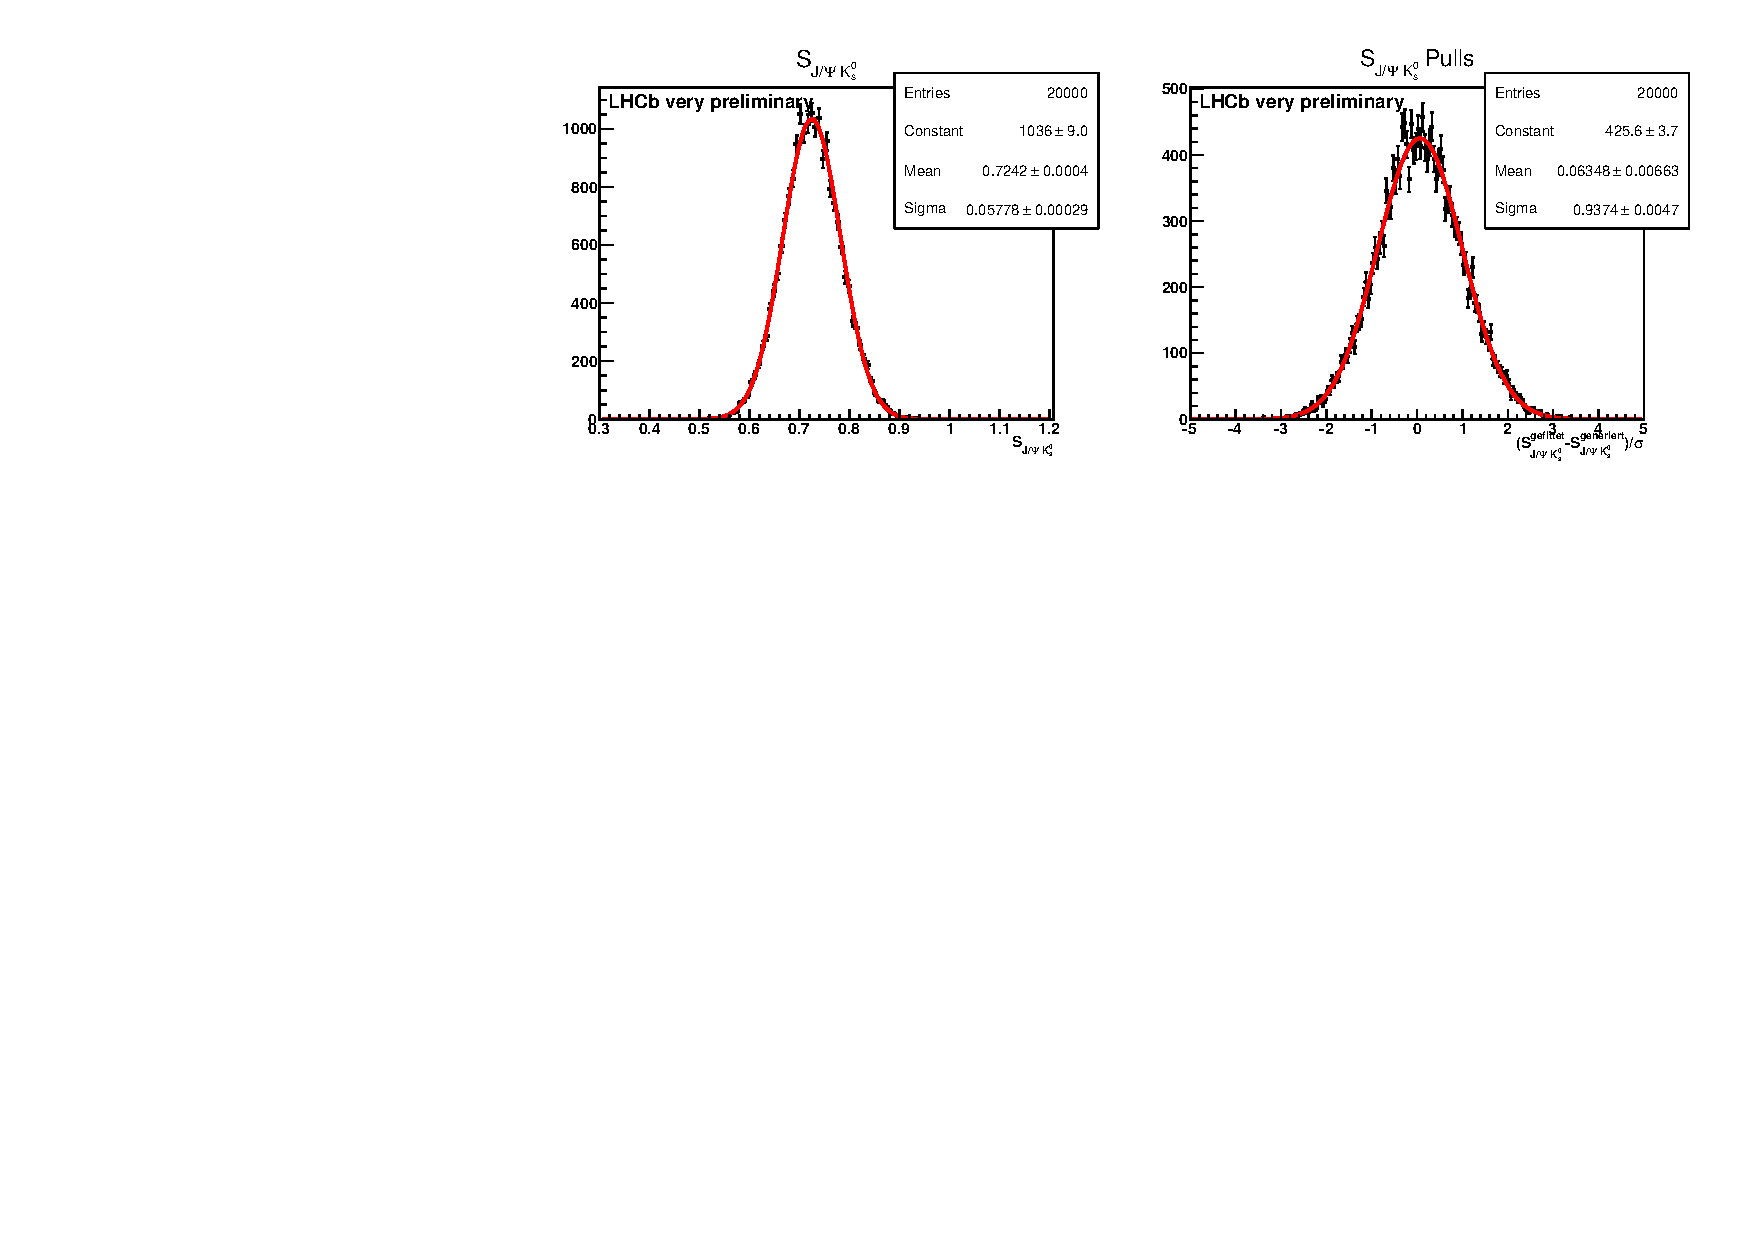
\includegraphics[width = \textwidth]{time_acceptance_toys}
\caption{Untersuchung des Einflusses einer zeitlichen Akzeptanz: Verteilung der aus der Toy MC Studie erhaltenen Amplituden $\SJPsi$ (links) sowie die dazugehörigen Pulls (rechts)}
\label{fig:toys_acceptance}
\end{figure}

Der Mittelwert der Amplitudenverteilung beträgt $\SJPsi = 0,72420 \pm 0,00041$. Die Abweichung vom Referenzwert (Fit Bias, siehe Kap. \ref{kap:fit_bias} $\SJPsi = 0,72343 \pm 0,00041$,
\begin{align}
\delta\SJPsi^{\text{Akz.}} = 0,00077\,
\end{align}
wird zur Abschätzung des Fehlers durch Vernachlässigung einer Akzeptanzfunktion verwendet. Gerade im Vergleich zum Einfluss des Flavour Taggings auf $\SJPsi$ ist dieser hier sehr gering. Somit erscheint das Vorgehen, keine Akzeptanz im Eigenzeitfit zu verwenden, gerechtfertigt.


\section{Korrelation zwischen Masse und Eigenzeit}
Die sFit-Methode funktioniert dann gut, wenn der Untergrund der Massenverteilung eben ist und die Massenverteilung des Signals unabhängig von der gemessenen Eigenzeit ist. Es soll nun eine etwaige Korrelation zwischen Masse und Eigenzeit untersucht und der Einfluss auf $\SJPsi$ festgestellt werden. Dazu wird die Massenverteilung in vier verschiedenen Zeitbereichen gefittet, die Tabelle \ref{tab:mass_ct} zu entnehmen sind. Anschließend wird die gesamte Eigenzeitverteilung gefittet, dabei werden aber die Massenparameter des Signals auf die in den 4 Massenfits erhaltenen Werte fixiert. Die Ergebnisse des jeweiligen Fits sind ebenfalls in Tabelle \ref{tab:mass_ct} aufgeführt.

\begin{table}[hptb]
\centering
\caption{Einteilung der Eigenzeitbereiche sowie Fitresultate für $\SJPsi$ bei Fixierung der Masse auf die in den Zeitbereichen enthaltene Massenform. Weiterhin werden die Abweichung $\Delta\SJPsi$ vom regulären Datenfit und der Signalanzahl $N_{sig}$ eines jeden Eigenzeitbereichs genannt.}
\label{tab:mass_ct}
\begin{tabular}{c l r@{$\pm$}l c c}
\hline \hline
Nr. & Eigenzeitfenster des Massenfits & \multicolumn{2}{c}{$\SJPsi$} & $\Delta\SJPsi$ & $N_{sig}$\\ \hline
1 & $t \in [0.3, 0.7] \pico\second$ & 0,5318 & 0,0626 & -0,0029 & 2882 \\
2 & $t \in [0.7, 1.5] \pico\second$ & 0,5361 & 0,0625 & 0,0014 & 4066 \\
3 & $t \in [1.5, 3] \pico\second$ & 0,5361 & 0,0625 & 0,0014 & 4230 \\
4 & $t \in [3, 14] \pico\second$ & 0,5353 & 0,0624 & 0,0006 & 2177 \\ \hline \hline
\end{tabular}
\end{table}

Zur Abschätzung des Fehlers werden zunächst die Abweichungen $\Delta\SJPsi$ vom (noch verdeckten) Referenzwert aus dem regulären Eigenzeitfit $\SJPsi = 0,5347 \pm 0,0626$ berechnet (siehe Kap. \ref{kap:fitergebnis} und diese dann - gewichtet nach der Signalzahl $N_{sig}$ eines jeden Bereichs - quadratisch gemittelt:
\begin{align}
\delta\SJPsi^{m/t} = \sqrt{\frac{\sum N_i (\Delta\SJPsi)_i}{\sum N_i}} = 0,0018
\end{align}

\section{Eigenzeitauflösung} \label{kap:aufloesung}
Bei einer effektiven Eigenzeitauflösung von $\sigma_{eff} = (0,0665 \pm 0,0013)\ps$ im Vergleich zur \Bd-Oszillationsfrequenz $\delta m_d = (0,521 \pm 0.039)\hbar\ps$ erwartet man keine nennenswerten Effekte auf die Amplitude $\SJPsi$. Um überhaupt einen Effekt zu sehen, werden die Auflösungsparameter $\sigma_i$ um 20\% ihres Werte erhöht bzw. gesenkt und damit dann der Datensatz gefittet. Die größte Abweichung vom Referenzwert des regulären Eigenzeitfits wird als systematischer Fehler angenommen. Die Ergenisse finden sich in Tabelle \ref{tab:syst_resolution}.

\begin{table}[hptb]
\centering
\caption{Ergebnisse des Eigenzeitfits bei Variaton der Auflösungsparameter $\sigma_i$ um $\pm 20\%$.}
\label{tab:syst_resolution}
\begin{tabular}{l c c c r@{$\pm$}l r }
\hline \hline
Variation & $sigma_1$ & $sigma_2$ & $sigma_3$ & \multicolumn{2}{c}{$\SJPsi$} & $\Delta\SJPsi$ \\ \hline
$+20\%$ & 0,576 & 0,05275 & 0,1118 & 0,5351 & 0,0626 & 0,0004 \\
$-20\%$ & 0,384 & 0,03517 & 0,0746 & 0,5345 & 0,0625 & -0,0002 \\ \hline \hline
\end{tabular}
\end{table}

Es zeigt sich, dass eine exakte Bestimmung der Auflösung nicht von Nöten ist, da sie im Vergleich zu anderen Systematiken vor allem gegenüber der Flavour-Tagging Kalibration vernachlässigt werden kann. Dennoch wird ein sytematischer Fehler durch die Auflösung mit
\begin{align}
\delta\SJPsi^{\text{Res.}} = 0,0004
\end{align}
assoziiert.

\section{Gesamtsystematik}
Tabelle \ref{tab:syst_gesamt} fasst nochmals alle systematischen Unsicherheiten zusammen. Der Gesamtfehler wird durch quadratische Addition berechnet.

\begin{table}[hptb]
\centering
\caption{Zusammenfassung der systematischen Unsicherheiten}
\label{tab:syst_gesamt}
\begin{tabular}{l c }
\hline \hline
Effekt & $\delta\SJPsi$ \\ \hline
Fitmethode & 0,0033 \\
Flavour-Tagging Kalibration & 0,0331 \\
Eigenzeitakzeptanz & 0,0008 \\
Korrelation Masse $\leftrightarrow$ Eigenzeit & 0,0018 \\ 
Eigenzeitauflösung & 0,0004 \\ \hline 
Gesamt & 0,0333 \\ \hline \hline
\end{tabular}
\end{table}
Es ist deutlich zu erkennen, dass die Kalibration der Flavour-Tagging-Algorithmen die dominierende Systematik ist. Obwohl hier zur Abschätzung der Systematik Werte der 2011-Kalibration genommen werden mussten, wird sich an dieser Tatsache nicht viel ändern, sobald diese Untersuchung mit Werten aus 2012 wiederholt wurde. Der systematischen Fehler von $\delta\SJPsi^{\text{stat.}}=0,0333$ ist nur etwa halb so groß wie der statistische $\delta\SJPsi^{\text{syst.}}=0,0626$. Damit ist definitiv noch Potential da, die Präzision durch mehr Datennahme zu verbessern.